\documentclass{article}


%%%% packages and definitions (optional)
\usepackage{graphicx} % allows inclusion of graphics
\usepackage{graphics}
\usepackage{placeins}
\usepackage{booktabs} % nice rules (thick lines) for tables
\usepackage{microtype} % improves typography for PDF


\usepackage{xcolor, colortbl}
\definecolor{Lightred}{rgb}{1.92,0.81,0.82}
\newcolumntype{a}{>{\columncolor{Lightred}}c}
\definecolor{LightCyan}{rgb}{0.88,1,1}
\newcolumntype{q}{>{\columncolor{LightCyan}}c}

\newcommand{\SN}{S$_N$}
\renewcommand{\vec}[1]{\bm{#1}} %vector is bold italic
\newcommand{\vd}{\bm{\cdot}} % slightly bold vector dot
\newcommand{\grad}{\vec{\nabla}} % gradient
\newcommand{\ud}{\mathop{}\!\mathrm{d}} % upright derivative symbol
\graphicspath{ {images/} }


%%%% Acronym support

\usepackage[acronym,toc]{glossaries}
\newacronym{NNL}{NNL}{National Nuclear Laboratory}
\newacronym{MA}{MA}{minor actinide}
\newacronym{DU}{DU}{depleted uranium}
\newacronym{LWR}{LWR}{Light Water Reactor}
\newacronym{MOX}{MOX}{Mixed Oxide Fuel}
\newacronym{SFR}{SFR}{Sodium-cooled Fast Reactor}
\newacronym{FLM}{FLM}{Fuel Loading Model}
\newacronym{EFMC}{EFMC}{Effective fissile mass coefficient}
\newacronym{ORNL}{ORNL}{Oak Ridge National Laboratory}
\newacronym{PWR}{PWR}{Pressurized Water Reactor}
\newacronym{FIT}{FIT}{Functionality Isolation Test}

\makeglossaries

%%%%%%%%%%%%%%actual words%%%%%%%%%%%%%%%%%%%%%%%%%%%%%%%%%%%%%%%%%%%%%%%%%%%%5
\begin{document}
\begin{titlepage}
    \centering
    {\scshape\LARGE ORION Functionality Isolation Test 1  \par}
    \vspace{1cm}
    {\scshape\Large Fuel Fabrication and Depletion Model\par}
    \vspace{2cm}
    {\Large\itshape Jin Whan Bae, Eva E. Davidson, 
    
    Joshua L. Peterson-Droogh, Andrew Worrall \par}
    \vfill
    Oak Ridge National Laboratory, Oak Ridge, TN
    \vfill
    \vfill

% Bottom of the page
    {\large \today\par}
\end{titlepage}




\section{Introduction}
The \gls{FIT} Benchmark is an international effort for better collaboration and testing of
various fuel cycle codes in use today. In this report, \gls{ORNL}'s contribution
to the \gls{FIT} Benchmark is discussed.

\gls{ORNL} analysts use ORION to perform various types of fuel cycle analyses.
ORION \cite{gregg_benefits_2013} is a systems dynamics analysis tool developed and maintained at \gls{NNL}.
It can simulate the full range of nuclear-related facilities, including storage, fabrication, enrichment,
and reprocessing facilities, as well as reactors. The facilities are connected on a canvas to form a
fuel cycle model, where the facilities are modeled as fleets. The code tracks over 2,500 nuclides
and models decay and in-reactor irradiation of fuel.

ORION in-reactor depletion calculations are performed with either cross sections or recipes.
Prior to an ORION analysis, detailed lattice physics calculations are completed to generate burnup-dependent
cross section libraries for ORION. The cross sections can be generated using lattice physics models set up in CASMO,
ECCO-ERANOS, FISPEN or SCALE. Stand-alone utility codes called SCORI and FISORI were developed and used to reformat
the one-group cross sections from SCALE into an ORION burnup-dependent cross section library format, hence loosely
coupling SCALE to ORION (shown in figure \ref{fig:sch}). These libraries are used in an ORION calculation using the MEEMS Pseudo Reactor (MPR) mode.
The MPR mode depletes the fuel by calculating the flux at a user-defined power density using quadratic interpolation,
 then solving the Bateman equation using the cross sections from the library. 

 \begin{figure}[htbp!]
    \begin{center}
    \resizebox{0.7\textwidth}{!}{
        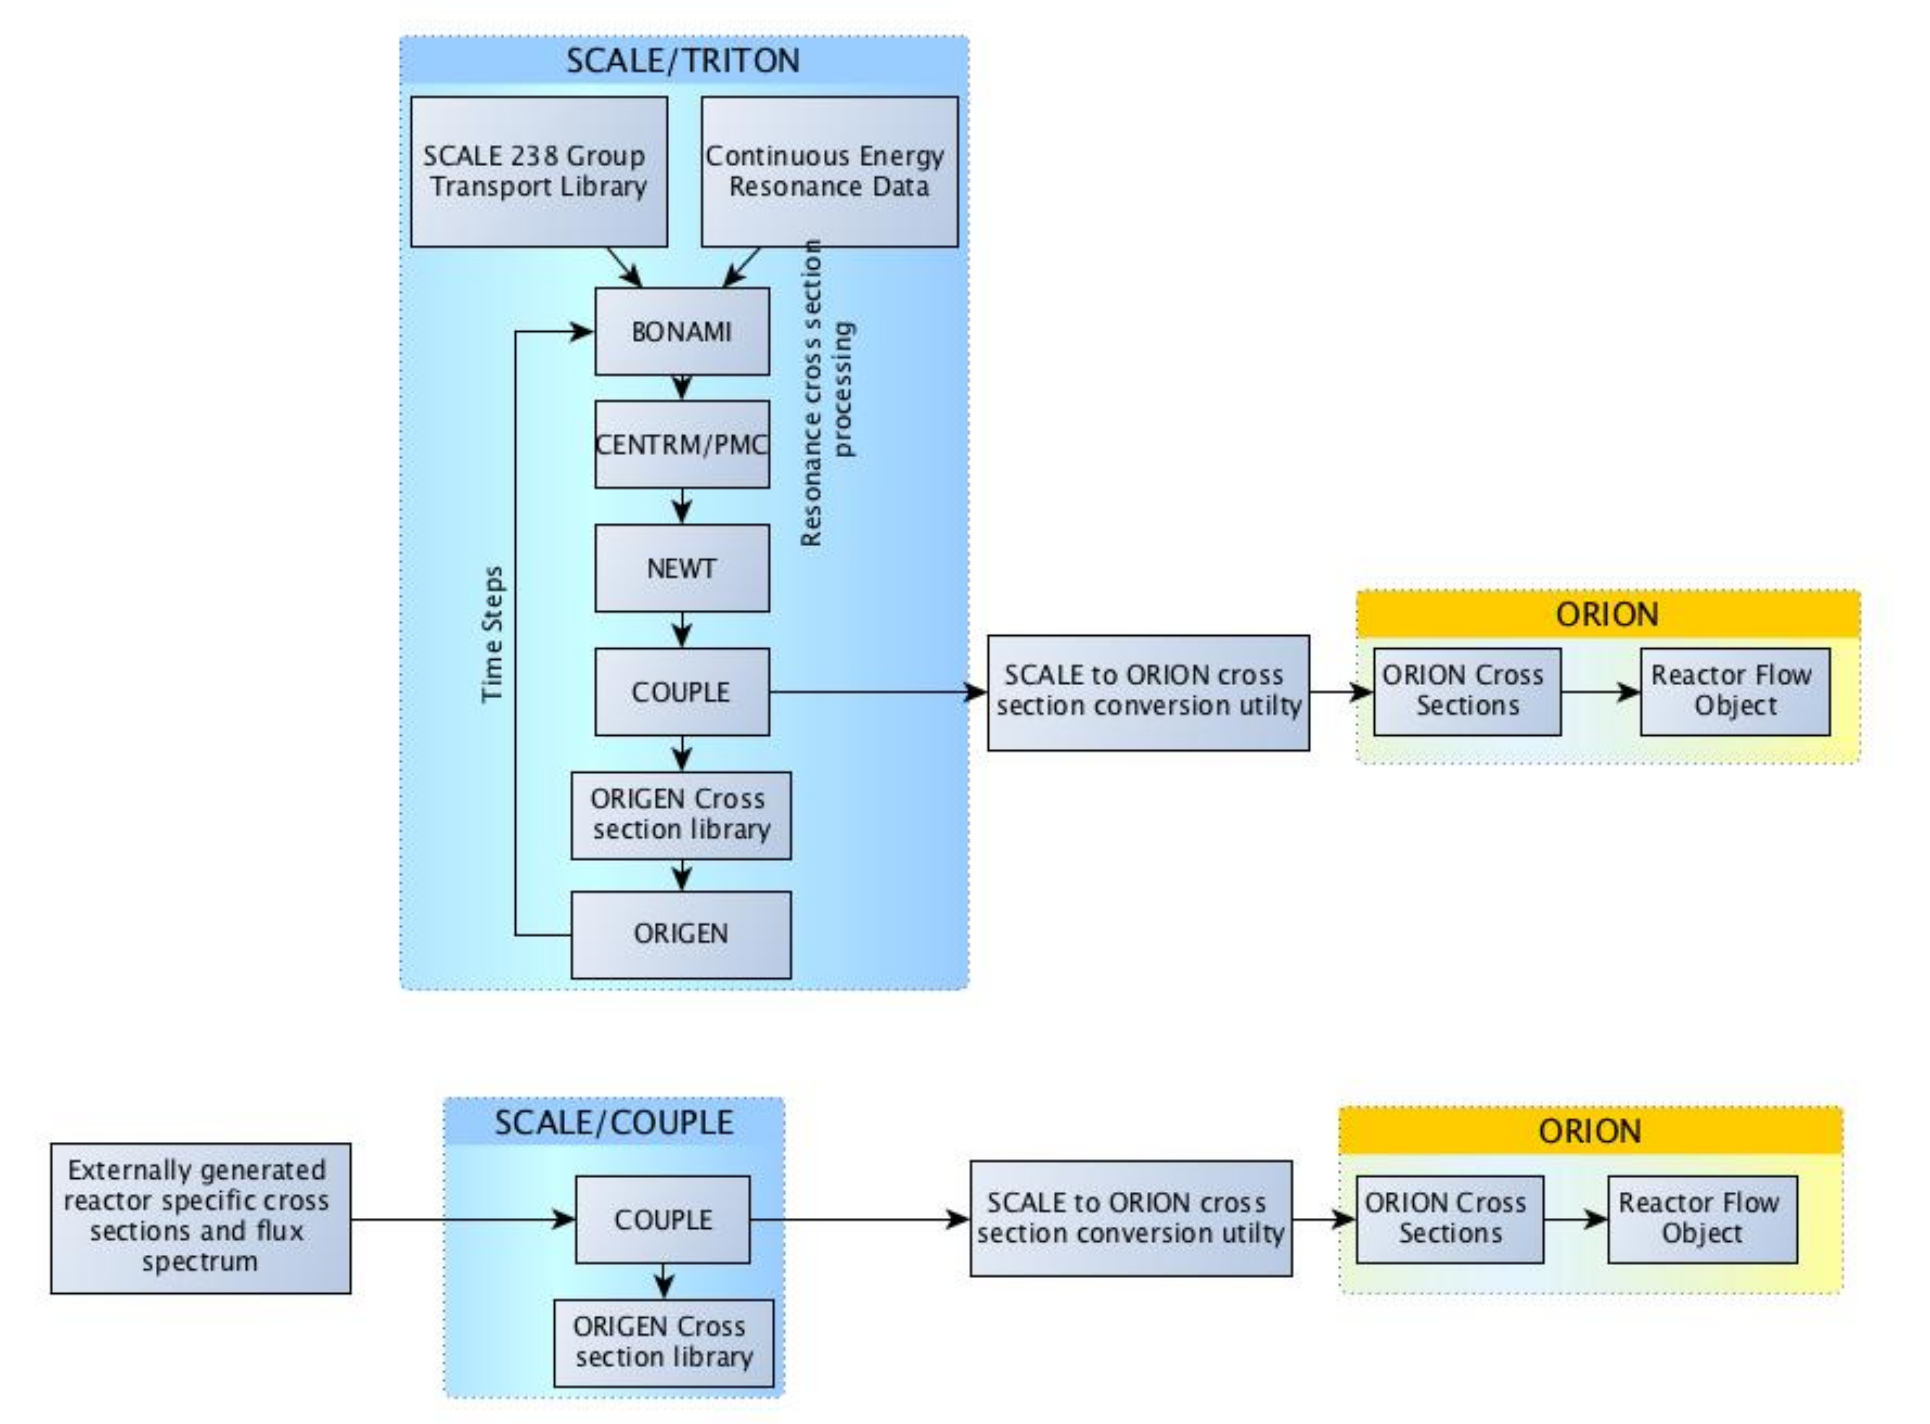
\includegraphics[scale=1.0]{./schematic.png}
        }
    \end{center}
    \caption{Schematic of link between SCALE and ORION}
    \label{fig:sch}
\end{figure}

In addition to generating cross sections, lattice physics codes can also be used to generate recipes, which are
tabulated isotopic fractions for a given fuel irradiation, used as transfer coefficients in ORION for each 
reactor and fuel type used. 


ORION  can potentially take advanced of \glspl{EFMC} to calculate how much of the fissile stream is needed. ORION reads
the absorption and fission cross section($\sigma_a, \sigma_f$) and the average number of neutrons produced per fission ($\nu$)
from the cross section data to calculate the equivalent fissile coefficient.

In this work, the \glspl{EFMC} has not been used to perform any analyses because the
cross section files available do not contain all the
input parameters required to generate these coefficients.
Furthermore, \gls{ORNL} has not tested this feature extensively and plans to perform tests
in the future with \glspl{EFMC}. Since the data available is insufficient to build the \glspl{EFMC}, only
the cross-section depletion approach is utilized to perform analyses for the \gls{FIT} benchmark and the results
are compared with the fixed fraction fuel compositions.



\section{Method}

A simple fuel cycle is created (shown in figure \ref{fig:flow}) where an \gls{MA} stream source
(plutonium and americium with predefined isotopic composition, shown in table \ref{tab:pu}) is mixed with a \gls{DU} (0.238\% $^{235}U$)
stream to create fuel for a single reactor. The two reactors tested are \gls{MOX} \glspl{PWR} (thermal spectrum), and \glspl{SFR} (fast spectrum). The reactor specifications
are listed in table \ref{tab:reac}. The fuel is then irradiated, using the MPR mode, to a predefined burnup and then sent to the buffer. We report the fuel composition going into the
reactor and out of the reactor. 

\begin{figure}[htbp!]
    \begin{center}
        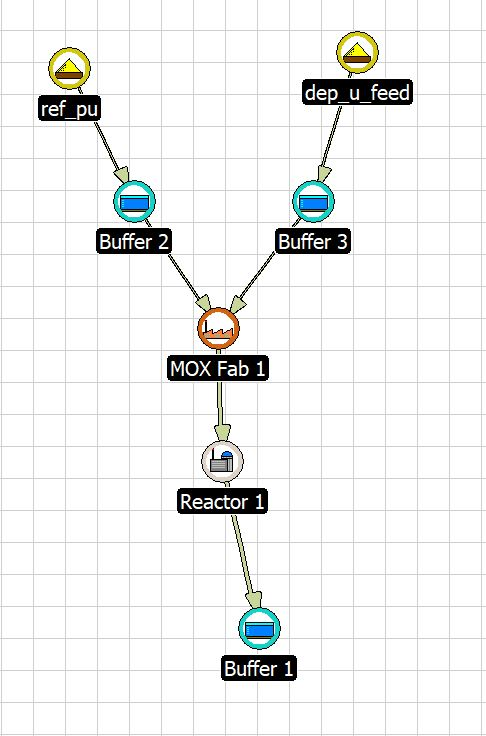
\includegraphics[scale=0.5]{./flow.jpg}
    \end{center}
    \caption{Material flow used for \gls{FIT} Benchmark.}
    \label{fig:flow}
\end{figure}

\begin{table}[htbp!]
    \centering
    \begin{tabular}{cccc}
        \hline
        Specification & Unit & \gls{MOX} \gls{PWR} & \gls{SFR} \\
        \hline
        Core Power & MWt & 3000 & 2500 \\
        Thermal Efficiency & \% & 30 & 40\\
        Capacity Factor & - & 0.9 & 0.9\\
        Cycle Length & year & 1 & 1.264\\
        Fuel Residence Time & year & 3.0 & 6.32 \\
        Number of Batches & - & 3 & 5\\
        Burnup & MWd/kgiHM & 41.09 & 100\\
        Core Inventory & kgHM/y & 72,000 & 51,953.4 \\
        \hline
    \end{tabular}
    \caption{Reactor specifications for the \gls{FIT} Benchmark.}
    \label{tab:reac}
\end{table}


\begin{table}[htbp!]
    \centering
    \begin{tabular}{c|cccc|cccc}
        \hline
        wt\% & \multicolumn{4}{c|}{\gls{MOX} \gls{PWR}} & \multicolumn{4}{c}{\gls{SFR}} \\
        \hline
        Isotope & ref & 1 & 2 & 3 & ref & 1 & 2 & 3 \\
        \hline
        Pu-238 &  0.48 & 3.12 & 3.32 & 4.00 & 1.98 & 3.12 & 2.87 & 4.00\\
        Pu-239 & 58.87 & 51.59 & 45.01 & 49.60 & 62.25 & 51.59 & 46.99 & 38.53 \\
        Pu-240 & 33.98 & 24.32 & 33.91 & 24.76 & 22.50 & 24.32 & 33.91 & 24.56 \\
        Pu-241 & 2.54 & 11.75 & 4.54 & 12.24 & 8.00 & 11.75 & 4.54 & 15.90 \\
        Pu-242 & 3.37 & 8.04 & 12.45 & 9.40 & 5.00 & 8.04 & 10.92 & 12.78 \\
        Am-241 & 0.77 & 1.18 & 0.77 & 0.78 & 0.27 & 1.18 & 0.77 & 4.23 \\
        \hline
    \end{tabular}
    \caption{\gls{MA} stream compositions for the \gls{FIT} Benchmark.}
    \label{tab:pu}
\end{table}

\subsection{Cross Section Generation}
For this test, we used a previously-generated cross section library as an input.
\gls{ORNL} has collaborated with \gls{NNL} to produce burnup-dependent cross section libraries specific to the fuel
cycles being evaluated in the FCO campaign \cite{wigeland_nuclear_2014}. The libraries are generated with the
SCALE suite of codes \cite{noauthor_scale_nodate}. The cross section for the \gls{PWR} \gls{MOX} model was generated from modeling
a Westinghouse 17 by 17 LOPAR fuel assembly in TRITON for 27 burnup steps and the cross section for the \gls{SFR}
model was generated from COUPLE using a steady-state flux spectrum from $MC^2-3 / REBUS-3$ \cite{lee_mc2-3:_2013}.
More details on cross section generation method can be found in Peterson et al \cite{peterson_generating_2016}. The
input compositions used for generating the cross sections are listed in table \ref{tab:inp}. Although ignored here, note that trace amounts
of other isotopes were used in generating the \gls{SFR}
driver and blanket cross sections in order to track
those isotopes.

\begin{table}[htbp!]
    \centering
    \begin{tabular}{c|ccc}
        \hline
        Isotopes & \gls{MOX} \gls{PWR} & \gls{SFR} Driver & \gls{SFR} Blanket  \\
        \hline
        U-235 & 0.22 & 0.108 & 0 \\
        U-238 & 91.9 & 82.5  & 100 \\
        Pu-238 & 0.122 & 0.033 & 0 \\
        Pu-239 & 4.703 & 13.1 & 0 \\
        Pu-240 & 2.009 & 3.33 & 0\\
        Pu-241 & 0.579 & 0.234 & 0 \\
        Pu-242 & 0.424 & 0.107 & 0 \\
        Am-241 & 0 & 0.113 & 0 \\
        \hline
        \hline
        Am+Pu & 7.83 & 16.8 & 0 \\
        \hline
    \end{tabular}
    \caption{Input composition used to generate cross sections for each reactor type.}
    \label{tab:inp}
\end{table}


\section{Results}
The results of the \gls{FIT} are reproduced below. Note that all the results are for the fixed fraction
fuel fabrication as discussed earlier. The depletion calculations are similar to the
results from other codes. The difference is calculated by the following equation:

\[ \text{\% diff } = \frac{\text{Cyclus result} - \text{ORION result}}{\text{Cyclus result}} * 100 \]

The main differences rise from the following two factors:

\begin{enumerate}
    \item Cross section generation methods and parameters
    \item `Lumping together' of driver and blanket region
\end{enumerate}

\subsection{\gls{MOX} \gls{LWR}}
Four qualities of \gls{MA} streams (ref, source one, two, three) are mixed with 
\gls{DU} (0.238\% $^{235}U$) in a fixed ratio (7\% \gls{MA}) and depleted in the thermal reactor
using the MPR mode in ORION. The charge and discharge fuel compositions are listed in
tables \ref{fig:lwr_charge} and \ref{fig:lwr_discharge}, respectively.  Note that an infinite percent difference
occur when the cyclus value is zero.

\begin{table}[h]
    \centering
    \resizebox{\textwidth}{!}{
    	\begin{tabular}{ccccc}
		\hline
		\textbf{wt\%} & \textbf{ref} & \textbf{source one} & \textbf{source two} & \textbf{source three} \\ 
		\hline
		U235 & 0.221 & 0.221 & 0.221 & 0.221 \\ 
		U238 & 92.77 & 92.77 & 92.77 & 92.77 \\ 
		PU238 & 0.138 & 0.218 & 0.200 & 0.279 \\ 
		PU239 & 4.357 & 3.611 & 3.289 & 2.697 \\ 
		PU240 & 1.574 & 1.702 & 2.373 & 1.719 \\ 
		PU241 & 0.559 & 0.822 & 0.317 & 1.112 \\ 
		PU242 & 0.349 & 0.562 & 0.764 & 0.894 \\ 
		AM241 & 0.018 & 0.082 & 0.053 & 0.296 \\ 
		Am+Pu & 6.999 & 6.999 & 6.999 & 6.999 \\ 
		\hline 
	\end{tabular} 
}
    \caption{Charge fuel composition for \gls{MOX} \gls{LWR} with percent differences from
             Cyclus results}
    \label{fig:lwr_charge}
\end{table}

\begin{table}[h]
    \centering
    \resizebox{\textwidth}{!}{
    	\begin{tabular}{c|ca|ca|ca|ca}
		\hline
		\textbf{wt\%} & \textbf{ref}  & \textbf{\% diff} & \textbf{1} & \textbf{\% diff} & \textbf{2} & \textbf{\% diff} & \textbf{3} & \textbf{\% diff}\\ 
		\hline
		\textbf{U234} & 0.002 & -4.07 & 0.002 & 33.14 & 0.003 & -4.35 & 0.005 & -4.89 \\ 
		\textbf{U235} & 0.117 & 0.065 & 0.108 & 5.815 & 0.099 & 6.339 & 0.099 & 8.988 \\ 
		\textbf{U236} & 0.023 & -1.03 & 0.024 & -2.50 & 0.026 & -6.29 & 0.026 & -6.32 \\ 
		\textbf{U238} & 90.51 & -0.40 & 89.89 & 0.193 & 89.85 & 0.051 & 89.86 & 0.076 \\ 
		\textbf{NP237} & 0.016 & -inf & 0.015 & -inf & 0.019 & -inf & 0.019 & -inf \\ 
		\textbf{PU236} & 0.0 & 0.0 & 0.0 & 0.0 & 0.0 & 0.0 & 0.0 & 0.0 \\ 
		\textbf{PU238} & 0.120 & 3.998 & 0.205 & 0.875 & 0.170 & 1.297 & 0.320 & 3.192 \\ 
		\textbf{PU239} & 2.255 & -0.55 & 2.175 & -10.7 & 1.836 & -5.43 & 1.760 & -5.97 \\ 
		\textbf{PU240} & 1.629 & -6.97 & 1.457 & 0.622 & 1.638 & 5.608 & 1.353 & -3.31 \\ 
		\textbf{PU241} & 0.862 & 4.373 & 0.910 & 1.680 & 0.953 & -1.49 & 0.863 & 4.151 \\ 
		\textbf{PU242} & 0.436 & 5.002 & 0.549 & 19.64 & 0.700 & 12.71 & 0.814 & 21.31 \\ 
		\textbf{AM241} & 0.059 & 5.982 & 0.078 & 2.161 & 0.069 & -8.99 & 0.116 & -0.51 \\ 
		\hline
		\hline
		\textbf{Am+Pu} & 5.486 & -3.19 & 5.592 & -4.95 & 5.611 & -2.83 & 5.526 & -3.21 \\ 
		\hline 
	\end{tabular} 
}
    \caption{Discharge fuel composition for \gls{MOX} \gls{LWR} with percent differences from
             Cyclus results}
    \label{fig:lwr_discharge}
\end{table}

\FloatBarrier

\subsection{\gls{SFR}}
Four qualities of \gls{SFR} streams (ref, source one, two, three) are mixed with
\gls{DU} (0.238\% $^{235}U$) in a fixed ratio (15.97\% \gls{MA}) and depleted in the 
fast reactor using the MPR mode in ORION. The charge and discharge fuel compositions are 
listed in tables \ref{fig:sfr_charge} and \ref{fig:sfr_discharge}, respectively.

Note that for the discharge compositions both the compositions depleted with driver
cross sections and blanket cross sections are listed in table \ref{fig:sfr_charge_only}.
This is because two separate
cross section data are acquired for ORION, but the \gls{SFR} specification in the
\gls{FIT} lumps the driver and blanket into one core. Given that difference, the depleted
composition should fall in between the depleted composition using the driver cross section (lower Pu+Am),
and the blanket cross section (higher Pu+Am).To prove this, we averaged the
obtained compositions by the mass fraction in the \gls{SFR} core. We assumed that
the driver fuel takes up 56.5\%, by referencing the \gls{PRISM} design \cite{triplett_prism:_2012}.
Then we compare this value to the Cyclus result, which has a difference of less than 10\% for all
isotopes, except for the traces isotopes such as U-236 and Pu-238.


\begin{table}[h]
    \centering
    \resizebox{\textwidth}{!}{
    	\begin{tabular}{ccccc}
		\hline
		\textbf{wt\%} & \textbf{ref} & \textbf{source one} & \textbf{source two} & \textbf{source three} \\ 
		\hline
		U235 & 0.199 & 0.199 & 0.199 & 0.199 \\ 
		U238 & 83.83 & 83.83 & 83.83 & 83.83 \\ 
		PU238 & 0.076 & 0.466 & 0.530 & 0.633 \\ 
		PU239 & 9.400 & 7.715 & 7.188 & 7.859 \\ 
		PU240 & 5.426 & 5.071 & 5.415 & 3.923 \\ 
		PU241 & 0.405 & 0.678 & 0.725 & 1.939 \\ 
		PU242 & 0.538 & 1.861 & 1.988 & 1.489 \\ 
		AM241 & 0.122 & 0.176 & 0.122 & 0.123 \\ 
		\hline
		\hline
		Am+Pu & 15.97 & 15.97 & 15.97 & 15.97 \\ 
		\hline 
	\end{tabular} 
}
    \caption{Charge fuel composition for \gls{SFR} with percent differences from
             Cyclus results}
    \label{fig:sfr_charge}
\end{table}


\begin{table}[h]
    \centering
    \resizebox{\textwidth}{!}{
    	\begin{tabular}{c|cc|cc|cc|cc}
		\hline
		\textbf{wt\%} & \textbf{ref driver} & \textbf{ref blanket} & \textbf{1 driver} & \textbf{1 blanket} & \textbf{2 driver} & \textbf{2 blanket} & \textbf{3 driver} & \textbf{3 blanket} \\ 		\hline
		\textbf{U234} & 0.002 & 6.149 & 0.012 & 0.012 & 0.013 & 0.013 & 0.017 & 0.017 \\ 
		\textbf{U235} & 0.079 & -10.2 & 0.090 & 0.058 & 0.088 & 0.057 & 0.094 & 0.063 \\ 
		\textbf{U236} & 0.025 & 14.81 & 0.021 & 0.032 & 0.021 & 0.032 & 0.019 & 0.031 \\ 
		\textbf{U238} & 75.24 & -3.18 & 76.30 & 72.79 & 76.18 & 72.61 & 76.72 & 73.53 \\ 
		\textbf{NP237} & 0.002 & 92.64 & 0.002 & 0.004 & 0.002 & 0.004 & 0.002 & 0.004 \\ 
		\textbf{PU236} & 0.0 & 0.0 & 0.0 & 0.0 & 0.0 & 0.0 & 0.0 & 0.0 \\ 
		\textbf{PU238} & 0.084 & 11.90 & 0.267 & 0.286 & 0.284 & 0.296 & 0.368 & 0.386 \\ 
		\textbf{PU239} & 9.113 & 5.824 & 7.684 & 9.503 & 7.461 & 9.342 & 7.783 & 9.559 \\ 
		\textbf{PU240} & 5.196 & 6.261 & 4.310 & 5.429 & 4.515 & 5.609 & 3.519 & 4.605 \\ 
		\textbf{PU241} & 0.629 & 5.681 & 0.537 & 0.819 & 0.569 & 0.859 & 0.841 & 0.928 \\ 
		\textbf{PU242} & 0.517 & -1.84 & 1.521 & 1.601 & 1.615 & 1.698 & 1.316 & 1.431 \\ 
		\textbf{AM241} & 0.155 & 7.982 & 0.201 & 0.186 & 0.180 & 0.174 & 0.300 & 0.245 \\ 
		\hline
		\hline
		\textbf{Am+Pu} & 15.75 & 5.413 & 14.67 & 18.10 & 14.78 & 18.27 & 14.24 & 17.38 \\ 
		\hline 
	\end{tabular} 
}
    \caption{Discharge fuel composition for \gls{SFR} using blanket and driver cross sections.}
    \label{fig:sfr_charge_only}
\end{table}

\begin{table}[h]
    \centering
    \resizebox{\textwidth}{!}{
    	\begin{tabular}{cccccccc}
		\hline
		\textbf{wt\%} & \textbf{ref blanket} & \textbf{ref driver} \textbf{one blanket} & \textbf{one driver} & \textbf{two blanket} & \textbf{two driver} & \textbf{three blanket} & \textbf{three driver} \\ 
		\hline
		U234 & 0.012 & 0.012 & 0.013 & 0.013 & 0.017 & 0.017 & 0.002 \\ 
		U235 & 0.090 & 0.058 & 0.088 & 0.057 & 0.094 & 0.063 & 0.092 \\ 
		U236 & 0.021 & 0.032 & 0.021 & 0.032 & 0.019 & 0.031 & 0.020 \\ 
		U238 & 76.30 & 72.79 & 76.18 & 72.61 & 76.72 & 73.53 & 76.66 \\ 
		Np237 & 0.0 & 0.0 & 0.0 & 0.0 & 0.0 & 0.0 & 0.0 \\ 
		PU236 & 0.0 & 0.0 & 0.0 & 0.0 & 0.0 & 0.0 & 0.0 \\ 
		PU238 & 0.267 & 0.286 & 0.284 & 0.296 & 0.368 & 0.386 & 0.072 \\ 
		PU239 & 7.684 & 9.503 & 7.461 & 9.342 & 7.783 & 9.559 & 8.415 \\ 
		PU240 & 4.310 & 5.429 & 4.515 & 5.609 & 3.519 & 4.605 & 4.692 \\ 
		PU241 & 0.537 & 0.819 & 0.569 & 0.859 & 0.841 & 0.928 & 0.485 \\ 
		PU242 & 1.521 & 1.601 & 1.615 & 1.698 & 1.316 & 1.431 & 0.479 \\ 
		AM241 & 0.201 & 0.186 & 0.180 & 0.174 & 0.300 & 0.245 & 0.152 \\ 
		Am+Pu & 14.67 & 18.10 & 14.78 & 18.27 & 14.24 & 17.38 & 14.34 \\ 
		\hline 
	\end{tabular} 
}
    \caption{Mass-averaged discharge fuel composition for \gls{SFR} with percent differences from
             Cyclus results}
    \label{fig:sfr_discharge}
\end{table}


\FloatBarrier

\section{Conclusion}
In-code fuel fabrication and depletion calculation capabilities are crucial
to modeling advanced fuel cycles.
Changes in the input stream can occur by multi-stage reprocessing or
technologies like on-line-reprocessing \glspl{MSR}. Using a fixed fraction method
for fuel fabrication and a recipe for depletion may work for a once-through cycle,
but can introduce large errors in advanced fuel cycles with input streams that change over time.

We tested ORION's capability to perform depletion calculations
using cross sections and a user-defined power density. We showed that
the change in plutonium stream quality does affect the ORION output depletion
from the reactor, and matches closely with the results from Cyclus.
However, the fuel loading model function in ORION is not tested
and is future work. Also, the \gls{SFR} discharge composition cannot be
compared directly, since the test \gls{SFR} uses a lumped-model \gls{SFR},
whereas the cross sections used for ORION separates the driver and the blanket fuel.
However, averaging the driver and blanket calculation to the mass fractions in the core
produces results close to the Cyclus result.

A better comparison could have been done if the analysts for different fuel cycle
codes used the same set of cross section data. However, it should be noted that
different codes use varying algorithms to perform fuel fabrication and depletion
calculations.


\bibliographystyle{unsrt}
\bibliography{bib}


\end{document}
